\section{Двухвыборочная задача}

Основное применение перестановочных тестов, и единственное, что мы обсуждаем здесь --- это двухвыборочная задача (8.3)--(8.5), в которой мы наблюдаем две независимые случайные выборки $\textbf{z} = (z_1, z_2, \ldots, z_n)$ и $\textbf{y} = (y_1, y_2, \ldots, y_m)$, взятые из возможно различных распределений вероятностей $F$ и $G$,
\begin{align}
	F \to \textbf{z} = (z_1, z_2, \ldots, z_n) \text{ независимо от} \notag \\
	G \to \textbf{y} = (y_1, y_2, \ldots, y_m).
\end{align}
Наблюдая за $\textbf{z}$ и $\textbf{y}$, мы хотим проверить \textit{нулевую гипотезу} $H_0$ об отсутствии разницы между $F$ и $G$
\begin{equation}
	H_0: F = G.
\end{equation}
Равенство $F = G$ означает, что $F$ и $G$ присваивают равные вероятности всем множествам, $\text{Prob}_F \{A\} = \text{Prob}_G \{A\}$ для $A$ любых подмножеств общего пространства выборок $z$ и $y$. Если $H_0$ истинно, то нет никаких различий между вероятностным поведением случайного $z$ или случайного $y$.

Проверка гипотез --- полезный инструмент для ситуаций, подобных ситуации с данными о мышах, таблица 2.1. Мы наблюдали небольшое количество данных, $n = 7$ экспериментальных измерений и $m = 9$ контрольных. Разница в средних
\begin{equation}
	\hat{\theta} = \bar{z} - \bar{y} = 30.63
\end{equation}
побуждает нас поверить в то, что распределение экспериментальных данных $F$ дает более продолжительное время выживания, чем распределение контрольных данных $G$. На самом деле эксперимент был разработан, чтобы продемонстрировать именно этот результат.

В этой ситуации \textit{нулевая гипотеза} (15.2) о том, что $F = G$, играет роль адвоката дьявола. Если мы не можем решительно отвергнуть возможность того, что $H_0$ истинно (как окажется в случае с данными о мышах), то мы не сможем успешно продемонстрировать превосходство лечения над не лечением. \textit{Проверка гипотезы}, примером которой и является перестановочный тест, представляет собой формальный способ решить, отвергают ли данные $H_0$ решительно.

Проверка гипотез начинается с \textit{тестовой статистики} $\hat{\theta}$, разности средних (15.3). Для удобства мы предположим, что если нулевая гипотеза $H_0$ не верна, мы ожидаем увидеть большие значения $\hat{\theta}$, чем если бы $H_0$ была верна. Если лечение работает лучше, чем не лечение в эксперименте с мышами, как и предполагалось, то мы ожидаем, что $\hat{\theta} = \bar{z} - \bar{y}$ будет большим. Нам не нужно количественно определять, что означает «большой», чтобы проводить проверку гипотезы. Все, что мы говорим, это то что, чем больше значение $\hat{\theta}$, которое мы наблюдаем, тем сильнее доказательства против $H_0$. Конечно, в других ситуациях мы могли бы выбрать меньшие значения вместо больших, чтобы представить более убедительные доказательства. Возможны и более сложные варианты, см. (15.26).

Наблюдаемый $\hat{\theta}$ (достигнутый уровень значимости теста, сокращенно ASL), определяется как вероятность наблюдения, по крайней мере, такого большого значения, когда нулевая гипотеза верна,
\begin{equation}
	\text{ASL} = \text{Prob}_{H_0} \{ \hat{\theta}^* \geq \hat{\theta} \}.
\end{equation}
Чем меньше значение ASL, тем сильнее доказательства против $H_0$, как подробно описано ниже. Величина $\hat{\theta}$ в (15.4) зафиксирована на своем наблюдаемом значении; случайная величина $\hat{\theta}^*$ имеет распределение нулевой гипотезы, распределение $\hat{\theta}$, если $H_0$ истинно. Как и раньше, в обозначениях со звездочкой указывается различие между фактическим наблюдением $\hat{\theta}$ и гипотетическим $\hat{\theta}^*$, сгенерированным в соответствии с $H_0$.

Проверка гипотезы $H_0$ состоит из вычисления ASL и проверки того, является ли оно слишком маленьким в сравнении с определенными стандартными пороговыми значениями. Формально мы выбираем малую вероятность $\alpha$, например $0.05$ или $0.01$, и \textit{отклоняем} $H_0$, если ASL меньше $\alpha$. Если ASL больше $\alpha$, то мы \textit{принимаем} $H_0$, что означает, что экспериментальные данные не отвергают решительно нулевую гипотезу (15.2) об отсутствии разницы между $F$ и $G$. Менее формально, мы наблюдаем ASL и оцениваем доказательства против $H_0$ в соответствии со следующими приблизительными соглашениями:
\begin{align}
	\text{ASL} <0.1 & \quad \text{слабо веские доказательства против } H_0; \notag \\
	\text{ASL} <0.05 & \quad \text{достаточно веские доказательства против } H_0; \notag \\
	\text{ASL} <0.025 & \quad \text{веские доказательства против } H_0; \notag \\
	\text{ASL} <0.01 & \quad \text{очень веские доказательства против } H_0.
\end{align}


Традиционная проверка гипотез для данных о мышах может начинаться с предположения, что $F$ и $G$ являются нормальными распределениями с возможно разными средними значениями
\begin{equation}
	F = N(\mu_T, \sigma^2), \quad G = N(\mu_C, \sigma^2).
\end{equation}
Нулевая гипотеза $H_0: \mu_T = \mu_C$· При $H_0$, $\hat{\theta} = \bar{z} - \bar{y}$ имеет нормальное распределение со средним 0 и дисперсией $\sigma^2 \left[ \dfrac{1}{n} + \dfrac{1}{m} \right]$,
\begin{equation}
	H_0: \hat{\theta} \sim N \left(0, \sigma^2 \left(\dfrac{1}{n} + \dfrac{1}{m}\right)\right),
\end{equation}
Наблюдая $\hat{\theta}$, ASL представляет собой вероятность того, что случайная величина $\hat{\theta}^*$, распределенная, как в (15.7), превышает $\hat{\theta}$,
\begin{equation}
	\text{ASL} = \text{Prob} \left\{ Z > \dfrac{\hat{\theta}}{\sigma \sqrt{1/n + 1/m} }\right\} = 1 - \Phi \left( \dfrac{\hat{\theta}}{\sigma \sqrt{1/n + 1/m}} \right),
\end{equation}
где $\Phi$ --- функция распределения стандартной нормальной переменной $Z$.

Мы не знаем $\sigma$. Стандартная оценка, основанная на (15.6)
\begin{equation}
	\bar{\sigma} = \left\{ \left[ \sum\limits_{i=1}^{n} (z_i - \bar{z})^2 + \sum\limits_{j=1}^{m} (y_j - \bar{y})^2 \right]/[n+m-2] \right\}^{\dfrac{1}{2}},
\end{equation}
что равно 54.21 для данных о мышах. Подставляя $\bar{\sigma}$ в (15.8) и помня, что $\hat{\theta} = 30.63$ дает
\begin{equation}
	\text{ASL} = 1 - \Phi\left(\dfrac{30.63}{54.21 \sqrt{1/9 + 1/7}}\right) = 0.131.
\end{equation}
При этом вычислении $\bar{\sigma}$ рассматривается как фиксированная константа. T-критерий Стьюдента, учитывающий случайность в $\bar{\sigma}$, дает
\begin{equation}
	\text{ASL} = \text{Prob} \left\{ t_{14} > \dfrac{30.63}{54.21 \sqrt{1/9 + 1/7}} \right\} = 0.141,
\end{equation}
$t_{14}$ указывает на статистику $t$ с $14$ степенями свободы. Тест Стьюдента основан на тестовой статистике $\hat{\theta}/[\bar{\sigma} \sqrt{1/n+1/m}]^{1/2}$ вместо $\hat{\theta}$. Эта статистика имеет распределение $t_{n+m-2}$ при нулевой гипотезе. В этом случае ни (15.10), ни (15.11) не позволяют нам отвергнуть нулевую гипотезу $H_0$ согласно (15.5) при всех стандартных уровнях значимости.

Основная практическая трудность при проверке гипотез заключается в вычислении ASL (15.4). Мы написали $\text{Prob}_{H_0} \{ \hat{\theta}^* > \hat{\theta} \}$, как если бы нулевая гипотеза $H_0$ задавала единственное распределение, из которого мы можем вычислить вероятность того, что $\hat{\theta}^*$ превысит $\hat{\theta}$. В большинстве задач нулевая гипотеза (15.2), $F = G$, оставляет нам семейство возможных распределений нулевых гипотез, а не только одно распределение. В нормальном случае (15.6), например, семейство нулевой гипотезы (15.7) включает в себя все нормальные распределения с математическим ожиданием 0. Чтобы фактически вычислить ASL, мы должны были либо аппроксимировать дисперсию нулевой гипотезы, как в (15.10), либо использовать Метод Стьюдента (15.11). Метод Стьюдента прекрасно решает проблему, но он применим только в случаях нормального распределения (15.6).

Перестановочный метод Фишера --- это разумный способ вычисления ASL для общей нулевой гипотезы $F = G$. Перед тем, как мы углубимся в подробности, приведем простое его описание. Если нулевая гипотеза верна, любое время выживания для любой из мышей может быть одинаково хорошим при любом из вариантов лечения. Итак, мы объединяем все $m + n$ наблюдений из обеих групп вместе, затем берем выборку размера $m$ без возвращения, чтобы представить первую группу; остальные $n$ наблюдений составляют вторую группу. Мы вычисляем разницу между средними значениями групп и затем повторяем этот процесс много раз. Если исходная разница в выборочных средних выходит за пределы средних 95\% распределения различий, двусторонний перестановочный тест отклоняет нулевую гипотезу на уровне 5\%.

Перестановочные тесты основаны на \textit{порядковом статистическом представлении} данных $\textbf{x} = (\textbf{z}, \textbf{y})$ из двухвыборочной задачи. В таблице 15.1 показано порядковое статистическое представление для данных о мышах из таблицы 2.1. Все 16 времен выживания были объединены и отсортированы от наименьшего к наибольшему. В нижней строке приведены ранжированные значения в диапазоне от наименьшего значения 10 до наибольшего значения 197. К какой группе принадлежит каждая точка данных, «$z$» для экспериментальной или «$y$» для контрольной группы, показано в верхней строке. Во второй строке показаны ранги с 1 по 16. Мы видим, например, что 11-е наименьшее значение в объединенном наборе данных имело место в экспериментальной группе и равнялось 94. Таблица 15.1 содержит ту же информацию, что и таблица 2.1, но организована таким образом, чтобы облегчить сравнение относительных размеров значений экспериментальной и контрольной групп.

Пусть $N$ равно объединенному размеру выборки $n + m$, и пусть $\textbf{v} = (v_1, v_2, \ldots, v_N)$ будет объединенным и упорядоченным вектором значений; $N = 16$ и $\textbf{v} = (10, 16, 23, \ldots, 197)$ для данных о мышах.\\
\noindent
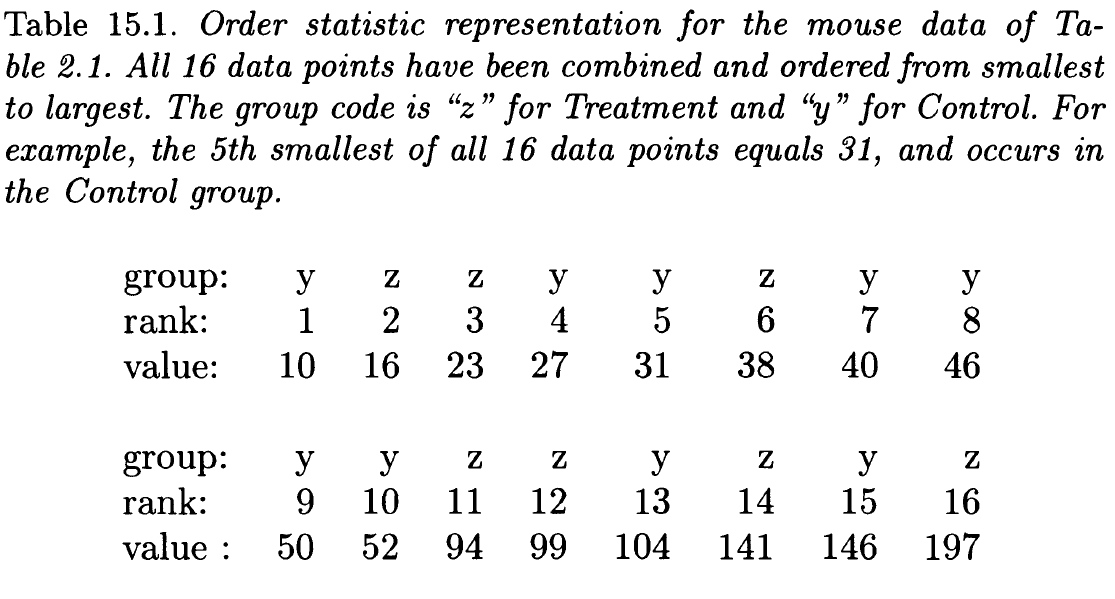
\includegraphics[width=\textwidth]{15/t15.1.png}
\newline
Также пусть $\textbf{g} = (g_1, g_2, \ldots, g_N)$ будет вектором, который указывает, к какой группе принадлежит каждое упорядоченное наблюдение, верхняя строка в таблице 15.1. Вместе $\textbf{v}$ и $\textbf{g}$ передают ту же информацию, что и $\textbf{x} = (\textbf{z}, \textbf{y})$.

Вектор $\textbf{g}$ состоит из $n$ значений z и $m$ значений y. Есть
\begin{equation}
	C_N^n = \dfrac{N!}{n!m!}
\end{equation}
возможных $\textbf{g}$ векторов, соответствующих всем возможным способам разбиения $N$ элементов на два подмножества размера $n$ и $m$. Перестановочные тесты зависят от следующего важного результата:\\
\underline{Лемма о перестановке}. \textit{При $H_0: F = G$ вектор $\textbf{g}$ с вероятностью $1/ C_N^n$ равняется любому из своих возможных значений}.\\
Другими словами, все перестановки $z$ и $y$ равновероятны, если $F = G$. Мы можем думать о тестовой статистике $\hat{\theta}$ как о функции от $\bf{g}$ и $\bf{v}$, скажем
\begin{equation}
	\hat{\theta} = S(\bf{g}, \bf{v}).
\end{equation}
Например, $\hat{\theta} = \bar{z} - \bar{y}$ можно выразить как
\begin{equation}
	\hat{\theta} = \dfrac{1}{n} \sum\limits_{g_i = z}^{} v_i - \dfrac{1}{m} \sum\limits_{g_i = y}^{} v_i,
\end{equation}
где $\sum_{g_i = z} v_i$ обозначает сумму $v_i$ по значениям $i = 1, 2, \ldots, N$, имеющим $g_i = z$.

Пусть $\bf{g}^*$ обозначает любой из $C_N^n$ возможных векторов состоящих из $n$ значений $z$ и $m$ значений $y$ и определяет \textit{перестановочные репликации} значения $\hat{\theta}$,
\begin{equation}
	\hat{\theta}^* = \hat{\theta}(\bf{g^*}) = S(\bf{g}^*, \bf{v}).
\end{equation}
Имеется $C_N^n$ перестановочных репликаций $\hat{\theta}^*$. Распределение, которое имеет вероятность $1/C_N^n$ для важдого каждый из них, называется \textit{перестановочным распределением} $\hat{\theta}$ или \textit{перестановочным распределением} $\hat{\theta}^*$. Перестановочный ASL определяется как перестановочная вероятность того, что $\hat{\theta}^*$ превышает $\hat{\theta}$,
\begin{equation}
	\text{ASL}_{\text{perm}} = \left\{ \text{Prob}_{\text{perm}} {\hat{\theta}^* \geq \hat{\theta}} \right\} = \# \{ \hat{\theta}^* \geq \hat{\theta} \} / C_N^n.
\end{equation}
Два определения $\text{ASL}_{\text{perm}}$ в (15.16) идентичны из-за леммы о перестановке.

На практике $\text{ASL}_\text{perm}$ обычно аппроксимируется методами Монте--Карло в соответствии с алгоритмом 15.1.

Перестановочный алгоритм очень похож на бутстреп алгоритм, показанный на рис. 6.1. Основное отличие состоит в том, что отбор проб осуществляется без повторения, а не с повторением.
\begin{center}
	Алгоритм 15.1
\end{center}
\noindent\fbox{\parbox{\textwidth}{
	\underline{Вычисление двухвыборочной перестановочной тестовой статистики.}
	
	1. Выберите $B$ независимых векторов $\textbf{g}^*(1), \textbf{g}^*(2),\ldots,\textbf{g}^*(B)$, каждый из которых состоит из $n$ значений $z$ и $m$ значений $y$ и каждый выбирается случайным образом из множества всех $C_N^n$ возможных таких векторов. [$B$ обычно составляет не менее 1000; см. таблицу (15.3).]
	
	2. Оцените перестановочные репликации $\hat{\theta}$, соответствующие каждому перестановочному вектору
	\begin{equation}
		\hat{\theta}^*(b) = S(\textbf{g}^*(b),v), \quad b = 1,2,\ldots,B.
	\end{equation}
	
	3. Оцениваем ASLperm
	\begin{equation}
		\widehat{\text{ASL}}_{\text{perm}} = \# \{ \hat{\theta}^*(b)\geq \hat{\theta} \}/B.
	\end{equation}
}}\\

На верхней левой части рисунка 15.1 показана гистограмма для $B = 1000$ перестановочных репликаций разности средни $\hat{\theta} = \bar{z} - \bar{y}$, (15.3); 132 из 1000 репликаций $\hat{\theta}^*$ превышают $\hat{\theta} = 30.63$, поэтому это подтверждает наш предыдущий вывод о том, что данные в таблице 2.1 не гарантирует отказ от гипотезы $F = G$
\begin{equation}
	\widehat{\text{ASL}}_{\text{perm}} = 132/1000 = 0.132.
\end{equation}
Перестановочный ASL близок к $t$-критерию ASL, (15.11), даже несмотря на то, что нет никаких предположений о нормальности, \textit{подчеркивающих} $\text{ASL}_{\text{perm}}$· Это не случайно, хотя очень небольшая разница между (15.19) и (15.11) отчасти случайна. Фишер продемонстрировал тесную теоретическую связь между перестановочным тестом на основе $\bar{z} - \bar{y}$ и критерием Стьюдента. Его основной целью при введении перестановочных тестов было поддержание использования теста Стьюдента в нестандартных приложениях.

\noindent
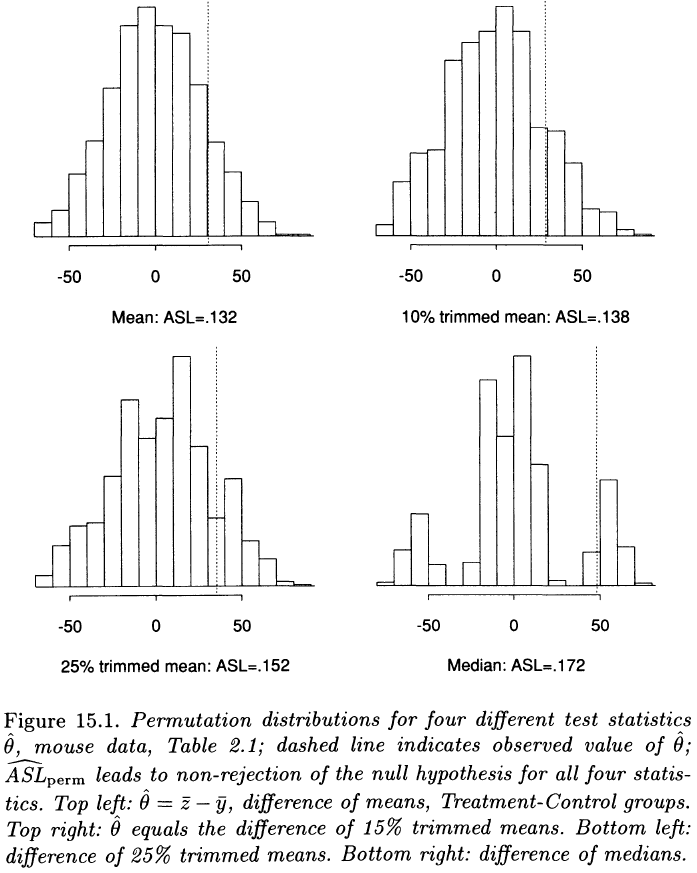
\includegraphics[width=\linewidth]{15/f15.1.png}
\newline

Сколько требуется перестановочных репликаций? Для удобного обозначения пусть $A = \text{ASL}_{\text{perm}}$ и $\hat{A} = \widehat{\text{ASL}}_{\text{perm}}$· Тогда $B \cdot \hat{A}$ равно количеству значений $\hat{\theta}^*(b)$, превышающих наблюдаемое значение $\hat{\theta}$, и поэтому имеет биномиальное распределение, как в задаче 3.6,
\begin{equation}
	B \cdot \hat{A} \sim \text{Bin}(B,A); \; \text{E}(\hat{A}) = A; \quad \text{var}(\hat{A}) = \dfrac{A(1-A)}{B}.
\end{equation}

\noindent
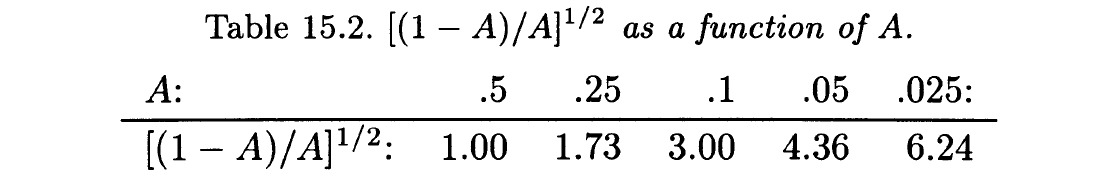
\includegraphics[width=\linewidth]{15/t15.2.png}
\newline

\noindent (Помните, что $\hat{\theta}$ является фиксированной величиной в (15.18), только $\hat{\theta}^*$ является случайным.) Коэффициент вариации $\hat{A}$ равен
\begin{equation}
	\text{cv}_B (\hat{A}) = \left[ \dfrac{(1-A)/A}{B} \right]^{1/2}.
\end{equation}
Величина $[ (1-A)/A ]^{1/2}$ становится больше по мере уменьшения $A$, как показано в таблице 15.2.

Предположим, мы требуем, чтобы $\text{cv}_B (\hat{A})$ было 0.10, что означает, что мы не хотим, чтобы ошибка Монте--Карло влияла на нашу оценку $\text{ASL}_\text{perm}$ более чем на 10\%. В таблице 15.3 указано количество требуемых перестановочных репликаций $B$.

Читателя может беспокоить особенность перестановочного тестирования: перестановочные репликации $\hat{\theta}^* = S(\bf{g}^*, \bf{v})$ изменяют часть исходных данных, но оставляют другую часть неизменной. Почему мы должны пересчитать $\bf{g}$, но не $\bf{v}$? В статистической литературе приводятся некоторые веские теоретические доводы, но основная причина --- практическая. «Условие на $\bf{v}$», то есть сохранение $\bf{v}$ фиксированным в перестановочном процессе сводит двухвыборочную ситуацию к \textit{единственному} распределению при нулевой гипотезе $F = G$. Это суть леммы о перестановке. Величина $\text{ASL}_\text{perm} = \text{Prob}_\text{perm} {\hat{\theta}^*> \hat{\theta}}$ четко определена, хотя, возможно, ее трудно вычислить, потому что $\text{Prob}_\text{perm}$ относится к уникальному распределению вероятностей. Величина $\text{ASL} = \text{Prob}_{H_0} {\hat{\theta}^* > \hat{\theta}}$ не определена должным образом, потому что не существует единого распределения $\text{Prob}_{H_0}$.

Самым большим достоинством перестановочного тестирования является ее точность. Если $H_0: F = G$ истинно, вероятность того, что $\text{ASL}_\text{perm}$ будет меньше 0.05, составляет почти 5\%. В общем виде
\begin{equation}
	\text{Prob}_{H_0} \{ \text{ASL}_\text{perm} < \alpha \} = \alpha
\end{equation}
для любого значения $\alpha$ от 0 до 1, за исключением небольших расхождений, вызванных дискретностью перестановочного распределения. Это важно, потому что интерпретирующая шкала (15.5) во многих областях применения понимается буквально.